\documentclass{article}
\usepackage[T1]{fontenc}
\usepackage{lmodern}
\usepackage{graphicx}
\usepackage{amsmath,amssymb}
\usepackage[a4paper,margin=2cm]{geometry}
\usepackage[absolute,overlay]{textpos}
\setlength{\TPHorizModule}{1mm}
\setlength{\TPVertModule}{1mm}
\usepackage[indonesian]{babel}
\usepackage{hyperref}
\setlength{\emergencystretch}{2em}
% unit: Halaman 54

\begin{document}

% === Halaman 54 (llm) ===

\section*{Contoh substitusi di dalam $block\ cipher$ DES:}

\begin{itemize}
    \item Misalkan 6-bit masukan adalah $\mathbf{110100}$

    Substitusi 6-bit masukan dengan menggunakan tabel substitusi (S-Box). Caranya: Nomor baris tabel (bit ke-1 dan bit ke-6) = 10 (baris 2)

\vspace{62.37mm}

    Nomor kolom tabel (bit ke-2, 3, 4, dan 5) = 1010 (kolom 10)
\end{itemize}

\vspace{20mm}

Jadi, substitusi untuk 110100 adalah $entry$ pada baris 2 dan kolom 10, yaitu entri bernillai 4 atau 0100 dalam biner.

% deskripsi: Tabel S-Box DES yang menunjukkan pemetaan baris dan kolom untuk proses substitusi, dengan sel baris 2 kolom 10 yang diarsir biru.
% bbox normalisasi: [0.1400, 0.4200, 0.9200, 0.6300]
\begin{textblock*}{163.80mm}(29.40mm,124.74mm)
\noindent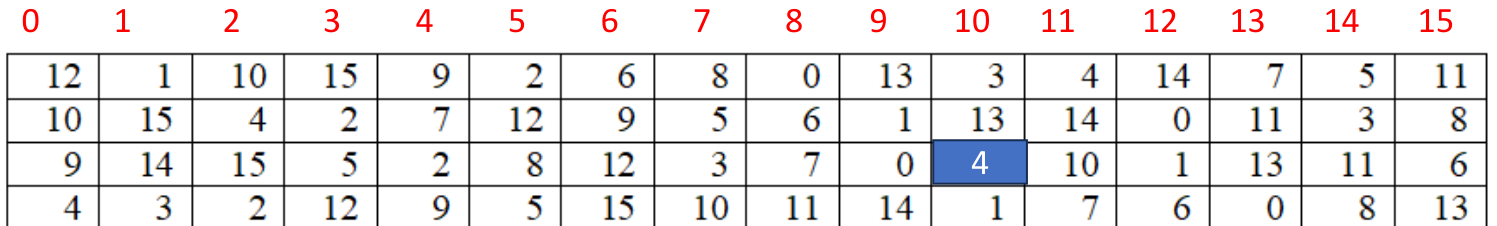
\includegraphics[width=163.80mm,height=62.37mm]{../../images/llm/page_054_img_01.png}%
\end{textblock*}

\end{document}
